\scanpage{89}
\mspage{95}

\diagram{\begin{tikzcd}[ampersand replacement=\&,row sep=large]
s_2\\
s_1\arrow[u,shift left=1.8pt,"p_1^{\deleted{\unsure{-|+|*}}}" ]\arrow[u,shift right=1.8pt,"p_1^+"' ]\\
s_0\arrow[u,shift left=1.8pt,"p_0^{\deleted{\unsure{-|+}}}" ]\arrow[u,shift right=1.8pt,"p_0^+"' ]
\end{tikzcd}}

avec

\[
\left\{\begin{aligned}p_1^-p_0^-&=p_1^-p_0^+\\p_1^+p_0^-&=p_1^+p_0^+\end{aligned}\right.
\]

\deleted{Mais prenons le produit de $I$ par le \deleted{\unsure{ens.}} \inserted{groupoïde trivial} à deux éléments \deleted{\unsure{$0,1$}}\inserted{$\{0,1\}$}, sur lequel $G$ opère librement,}

Mais prenons la subdivision barycentrique de la décomposition cellulaire précédente de $S$ \deleted{soit} dont les sommets correspondent aux \inserted{éléments de $\mathrm{Ob}\,I$, les simplexes, aux} parties totalement ordonnées de $\mathrm{Ob}\,I$. On trouve l'\uline{octaèdre}

\figure{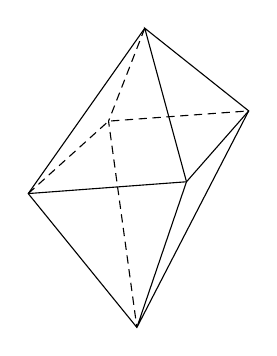
\begin{tikzpicture}[x=1cm,y=1cm]
\coordinate (t) at (1.48,2.1); \coordinate (b) at (1.38,-1.7);
\coordinate (l) at (0,0); \coordinate (r) at (2.8,1.05);
\coordinate (f) at (2.01,.15); \coordinate (h) at (1.02,.92);
\draw (t)--(l)--(b)--(r)--(t)--(f)--(b);
\draw (l)--(f)--(r); \draw[densely dashed] (t)--(h)--(b) (l)--(h)--(r);
\end{tikzpicture}}

\deleted{ayant 8 faces, \unsure{$4\times$}} ayant

\[
\begin{aligned}6&\text{ sommets}\\12&\text{ arêtes}\\8&\text{ faces}\end{aligned}
\]

et $G$ opère librement sur l'ens des simplexes, donc le quotient :

\[
\begin{aligned}3&\text{ sommets}\\6&\text{ arêtes}\\4&\text{ faces}\end{aligned}
\]

décomposition cellulaire du plan projectif. (Sa décomposition par trois droites.)

\figure{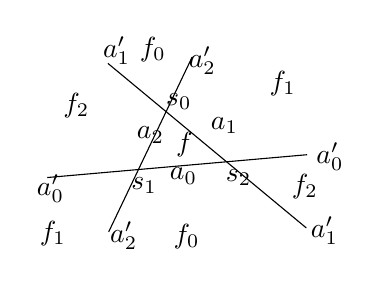
\begin{tikzpicture}[x=1cm,y=1cm]
\draw (-1.62,-.25)--(1.68,.04); \draw (-.84,-.94)--(.22,1.28); \draw (-.85,1.20)--(1.67,-.89);
\node at (-1.58,-.39) {$a'_0$}; \node at (1.97,.02) {$a'_0$};
\node at (-.74,1.36) {$a'_1$}; \node at (1.90,-.92) {$a'_1$};
\node at (.35,1.23) {$a'_2$}; \node at (-.65,-.99) {$a'_2$};
\node at (.05,.72) {$s_0$}; \node at (-.39,-.35) {$s_1$}; \node at (.81,-.25) {$s_2$};
\node at (.11,-.23) {$a_0$}; \node at (.63,.41) {$a_1$}; \node at (-.31,.29) {$a_2$};
\node at (.12,.17) {$f$}; \node at (-.28,1.38) {$f_0$}; \node at (.15,-1) {$f_0$};
\node at (1.37,.94) {$f_1$}; \node at (-1.55,-.96) {$f_1$};
\node at (-1.25,.67) {$f_2$}; \node at (1.65,-.36) {$f_2$};
\end{tikzpicture}}

On prend $S^1_{\deleted{\unsure{G|B}}}$ par l'ens. ordonné (comme au début)

\diagram{\begin{tikzcd}[ampersand replacement=\&,row sep=small,column sep=small]
s_1^-\&s_1^+\\ s_0^-\arrow[u]\arrow[ur]\&s_0^+\arrow[u]\arrow[ul]
\end{tikzcd}}

i.e.

\diagram{\begin{tikzcd}[ampersand replacement=\&,row sep=tiny,column sep=small]
\&s_1^+\&\\0=s_0^-\arrow[ur]\arrow[dr]\&\&s_0^+=0'\arrow[ul]\arrow[dl]\\
\&s_1^-\&
\end{tikzcd}}

et $G$ y opère, par symétrie échangeant $s_1^-$ et $s_{\unsure{1|i}}^+$. Donc \inserted{l'ens. ordonné} $X$ aura $4\times13=52$ sommets --- c'est \unsure{modeste|embêtant}\ldots

\figure{\begin{tikzpicture}[x=1cm,y=1cm]\draw (0,0) .. controls (.16,-.4) and (.55,-.87) .. (.83,-1.35); \draw (.68,-1.08)--(.66,-1.31);\end{tikzpicture}}

% archive sheet number: 88
